\chapter{Organic Light Emitting Diodes (OLEDs)}
\label{sec:bhj}

\begin{figure}[H]

\begin{tabular}{ c l }


\includegraphics[width=0.05\textwidth]{./images/youtube.png}

&
\href{https://www.youtube.com/watch?v=UPGc_GFWd-o}{Simulating OLEDs with multiple emission layers}
\\

\includegraphics[width=0.05\textwidth]{./images/youtube.png}

&
\href{https://www.youtube.com/watch?v=xhp_8e17tpU}{Simulating OLED structures using ray tracing and drift diffusion}
\\
\end{tabular}
\end{figure}

\section{Introduction}
Organic Light Emitting Diodes (OLEDs) are a widely used technology with applications in displays and sensing.  The devices operate by charge being injected through the contacts which results in electro luminescence. The following chapter describes how to simulate these devices using OghmaNano. There are various OLED examples which can be accessed from the OLED section of the \emph{New simulation window}a (Figure \ref{fig:oled1}).

\begin{figure}[H]
\centering
\begin{tabular}{ c c }

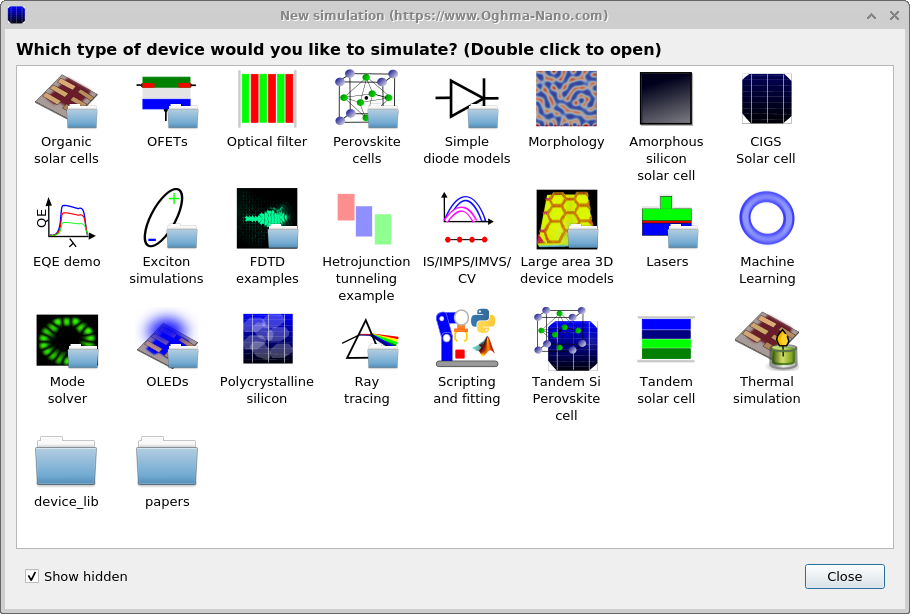
\includegraphics[width=0.5\textwidth,height=0.4\textwidth]{./images/oled/new_simulations.png}

&
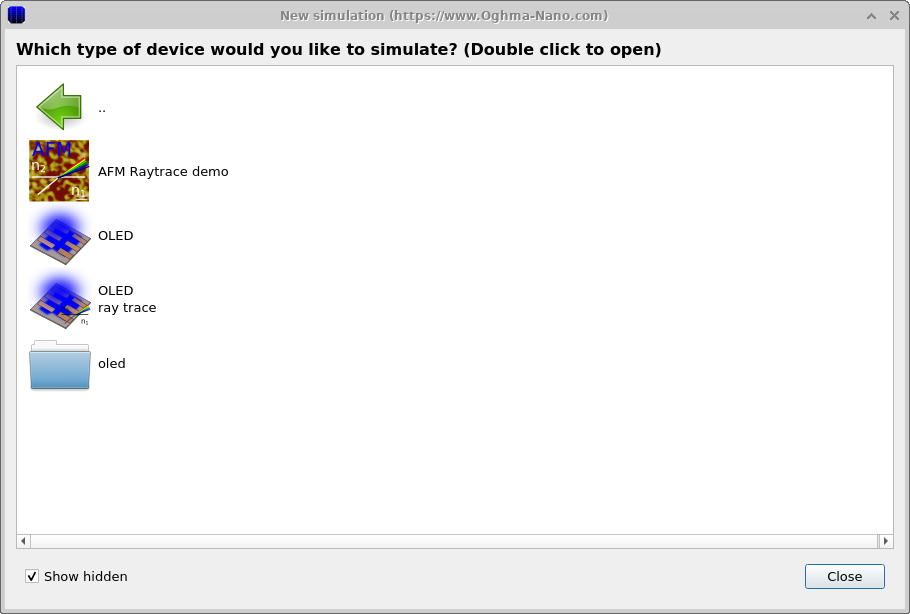
\includegraphics[width=0.5\textwidth,height=0.4\textwidth]{./images/oled/oled_new_sim.png}

\\
\end{tabular}
\caption{a) The new simulation window; b) OLED example simulations.}
\label{fig:oled1}
\end{figure}

OLED simulations use a combination of the drift-diffusion models described elsewhere in this book combined with optical models to simulate the propagation of light out of the device. The \emph{Transfer matrix method} and \emph{ray tracing} can be used to model the escape of light from OLEDs within OghmaNano. The transfer matrix method is useful when one wishes understand how light behaves when propagating normal to the surface of smoothed layer structures such as in well defined evaporated OLEDs, while the ray tracing method is used when wishing to simulate  light escaping from rough surfaces or structures with micro-lenses embedded.

\section{Optical outcoupling}
The most simple OLED simulation based on the transfer matrix method can be accessed by double clicking on the \emph{OLED} example simulation (see Figure \ref{fig:oled1}b). This will bring up the window shown in Figure \ref{fig:oled2}a. In the \emph{Optical} ribbon you will find a button called \emph{Optical outcoupling}. This tool allows the user to select which if the \emph{Transfer matrix method} or the \emph{ray tracing} method is used. If this window is opened a window resembling that shown in Figure \ref{fig:oled2}b will be displayed. By clicking \emph{Run} in this window, the probability of emission as a function of position and wavelength will be calculated this will be displayed in the \emph{Escape probability} tab. By clicking on \emph{Ray trace} and then clicking on the run button again, the simulation will be repeated using the ray tracing method, the results form such a simulation are shown in Figure \ref{fig:outcoupling_ray}. Note that the outcoupling efficiency for ray tracing is lower than that predicted by the transfer matrix as the transfer matrix method assumes propagation normal to the interfaces while ray tracing allows rays to travel in all directions some of which will never leave the device.

\begin{figure}[H]
\centering
\begin{tabular}{ c c }

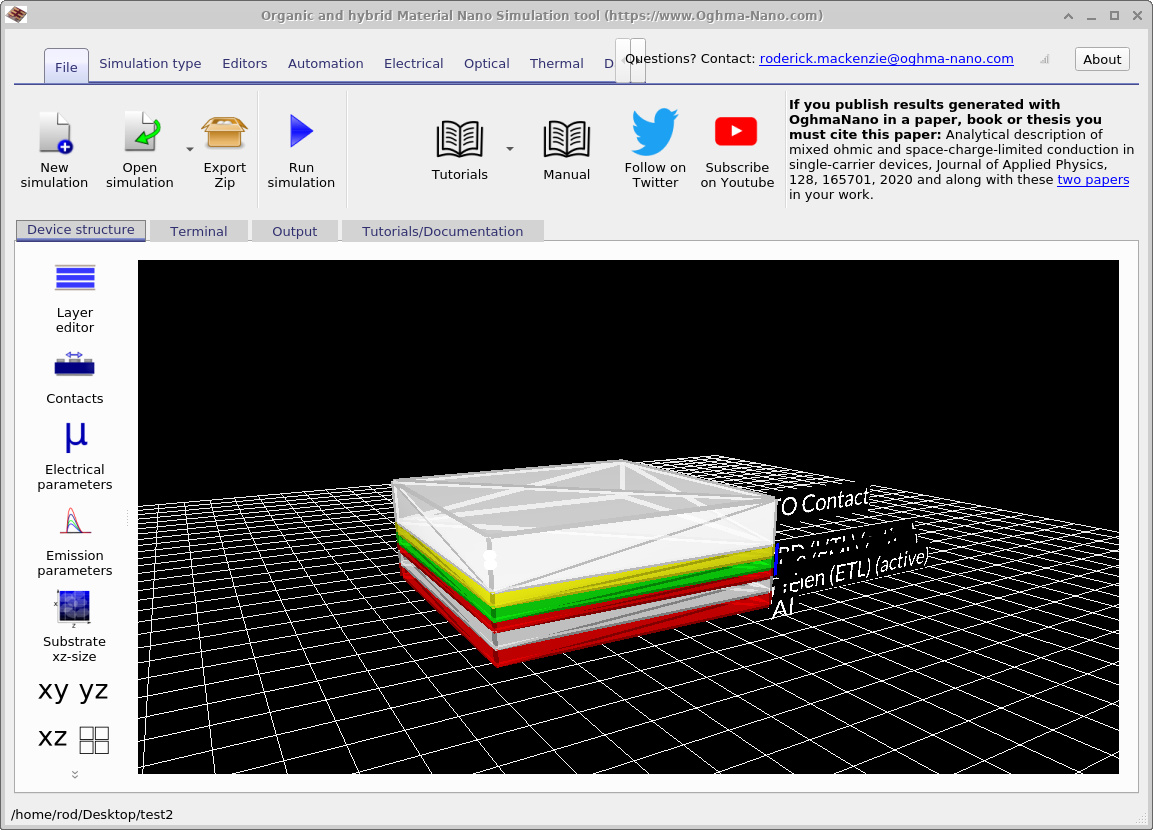
\includegraphics[width=0.5\textwidth,height=0.4\textwidth]{./images/oled/oled_start_example.png}

&
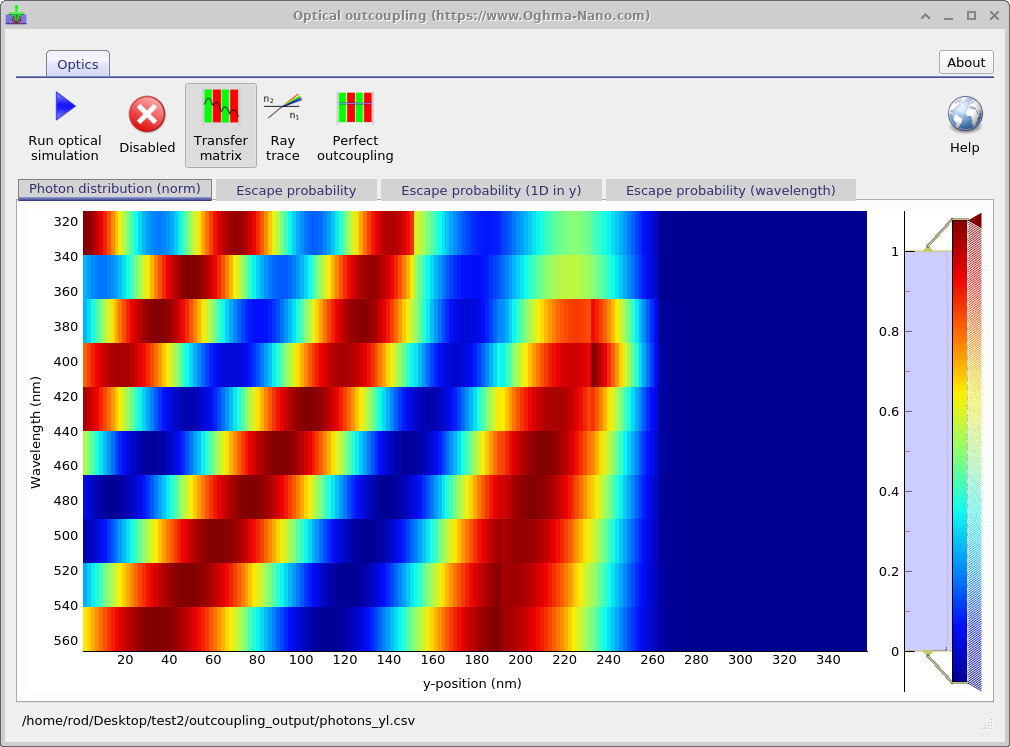
\includegraphics[width=0.5\textwidth,height=0.4\textwidth]{./images/oled/transfer_matrix.png}

\\
\end{tabular}
\caption{a) The OLED simulation; b) The results of an outcoupling simulation.}
\label{fig:oled2}
\end{figure}

\begin{figure}[H]
\centering
\begin{tabular}{ c c }

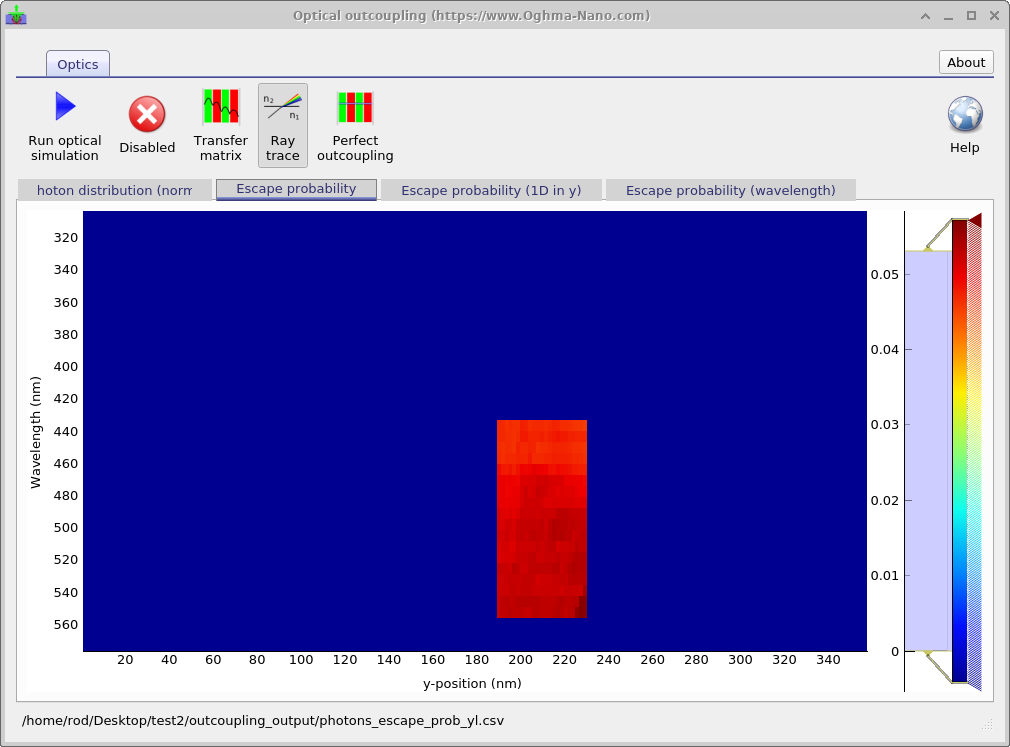
\includegraphics[width=0.5\textwidth,height=0.4\textwidth]{./images/oled/ray_trace_efficiency.png}

\\
\end{tabular}
\caption{a) Outcoupling calculated using ray the tracing method}
\label{fig:outcoupling_ray}
\end{figure}

\newpage
\section{Electrical simulations combined with optical transfer matrix calculations}
Make a new simulation based on the \emph{OLED} example as described above. Now run a full simulation by clicking on the \emph{Run simulation} button in the main window. This will run a full optical and electrical OLED simulation one after the other.  First an optical simulation will be performed to calculate what the probability of an emitted photon escaping the device will be at each electrical mesh point. Then a full Drift Diffusion simulation will be performed and the optical emission at each mesh point calculated form the recombination. The results will be shown in the \emph{Output} tab of the main window. The key files written to disk are described in table \ref{tab:oled_output}, examples of these files can be seen in Figures \ref{fig:li_and_eqe_curves}.

\begin{figure}[H]
\centering
\begin{tabular}{ c c }

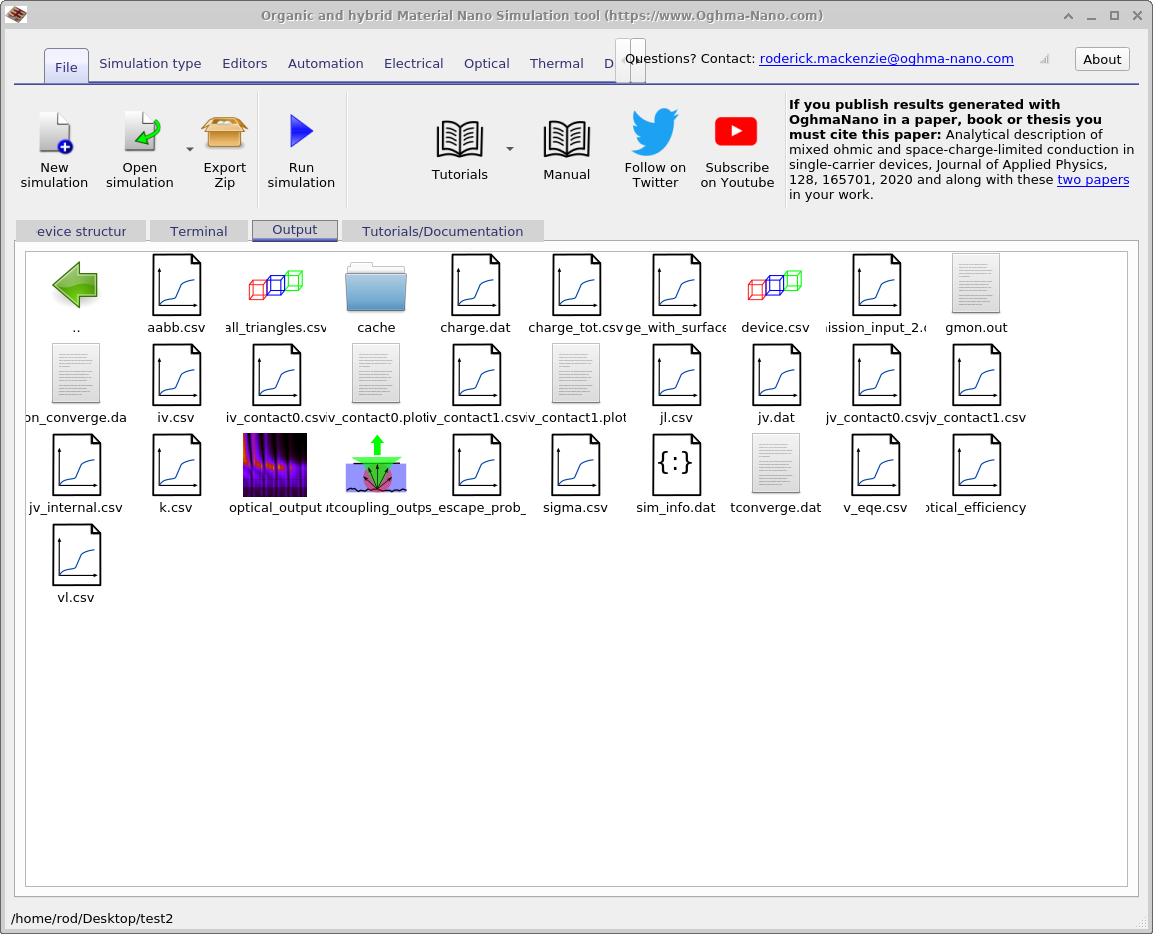
\includegraphics[width=0.5\textwidth,height=0.4\textwidth]{./images/oled/results.png}

\\
\end{tabular}
\caption{a) Out coupling calculated using ray the tracing method; b) }
\label{fig:oled3}
\end{figure}

\begin{table}[H]
\begin{center}
\begin{tabular}{ |c|l|c| } 
 \hline
	File name 			& 	Description  \\ 
 \hline
	$iv.csv$			&	Current v.s. voltage \\ 
	$jv.csv$			&	Current density v.s. voltage \\
	$jl.csv$			&	Current density v.s. optical output power density \\
	$k.csv$				&	Averaged recombination rate constant v.s. voltage \\
 	$v\_eqe.csv$		&	Voltage v.s. EQE\\
 	$vl.csv$			&	Voltage v.s. optical output power density\\
 	$Snapshots$			&	Snapshots of the electrical device parameters for each simulation step\\
 \hline
\end{tabular}
\caption{Key files produced by the OLED simulation.}
\label{tab:oled_output}
\end{center}
\end{table}

\begin{figure}[H]
\centering
\begin{tabular}{ c c }

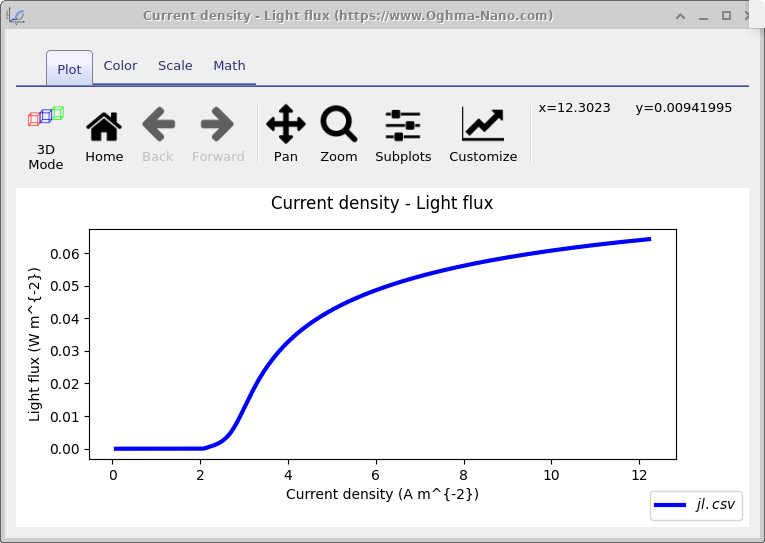
\includegraphics[width=0.5\textwidth,height=0.4\textwidth]{./images/oled/i_l.png}

&
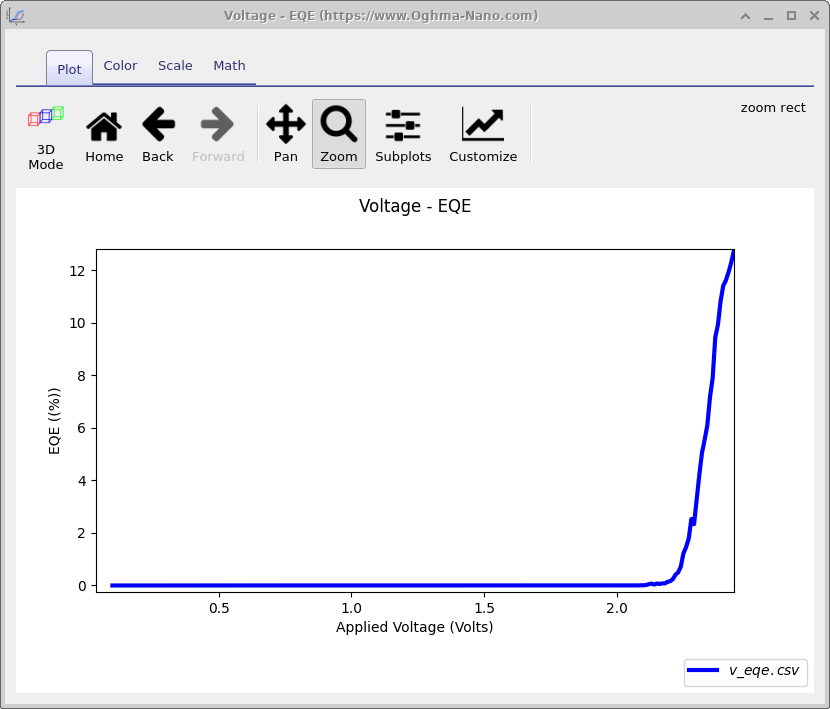
\includegraphics[width=0.5\textwidth,height=0.4\textwidth]{./images/oled/v_eqe.png}

\\
\end{tabular}
\caption{Example of the output from the OLED simulations of OghamNano}
\label{fig:li_and_eqe_curves}
\end{figure}

In the \emph{snapshots} directory you will find detailed electrical output from the model for each simulation step see Figure \ref{fig:oled4}. Also in that directory you will find a file entitled \emph{eqe.csv}. This contains the calculated EQE spectrum as a function of voltage. The EQE spectrum will change as the voltage changes because each point in the cavity of the device will have a different probability of outcoupling each wavelength of light to the world. As the carrier distribution in the device changes recombination will happen at different points  and thus the overall spectrum as observed from outside the device will change. Use the slider to see how the spectrum changes as a function of voltage.

\begin{figure}[H]
\centering
\begin{tabular}{ c c }

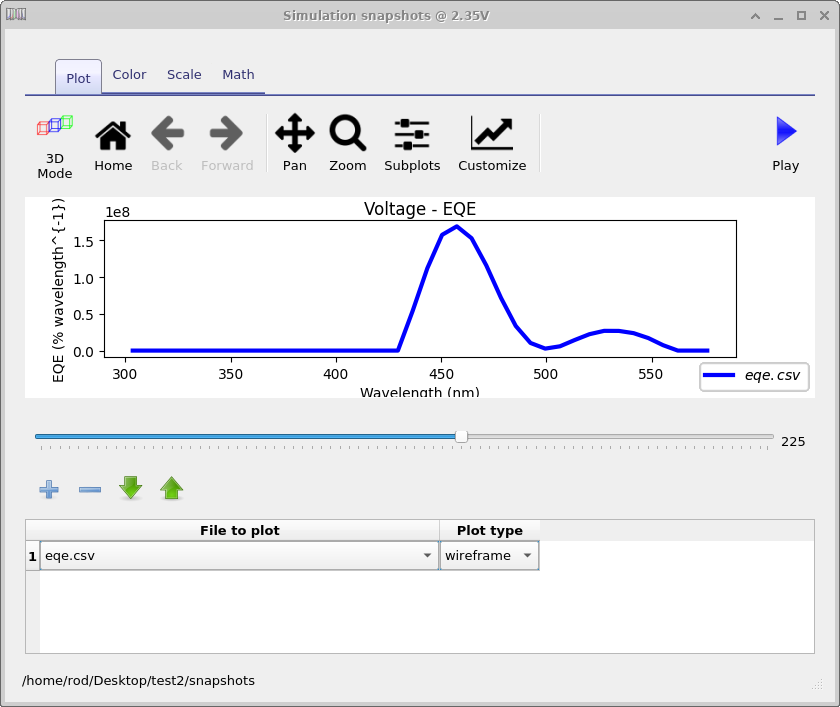
\includegraphics[width=0.5\textwidth,height=0.4\textwidth]{./images/oled/wavelength_eqe.png}

\\
\end{tabular}
\caption{The EQE spectrum calculated from the device in OghmaNano as a function of wavelength. The graph will change as applied voltage changes. To explore this use the slider in the window scroll over the results for various voltages}
\label{fig:oled4}
\end{figure}


\newpage
\section{Electrical simulations combined with ray tracing}

Ray tracing allows the user to tackle more complex optical problems such as when the device has rough surfaces, it also allows the user to examine rays that don't propagate normally to the interfaces. Two example ray tracing simulations are included \emph{AFM ray trace demo} and \emph{OLED ray trace}, these can be seen in Figure \ref{fig:oled5}a and the results of  \emph{AFM ray trace demo} can be seen in Figure \ref{fig:oled5}b note the rough surface of the OLED in this example.

\begin{figure}[H]
\centering
\begin{tabular}{ c c }

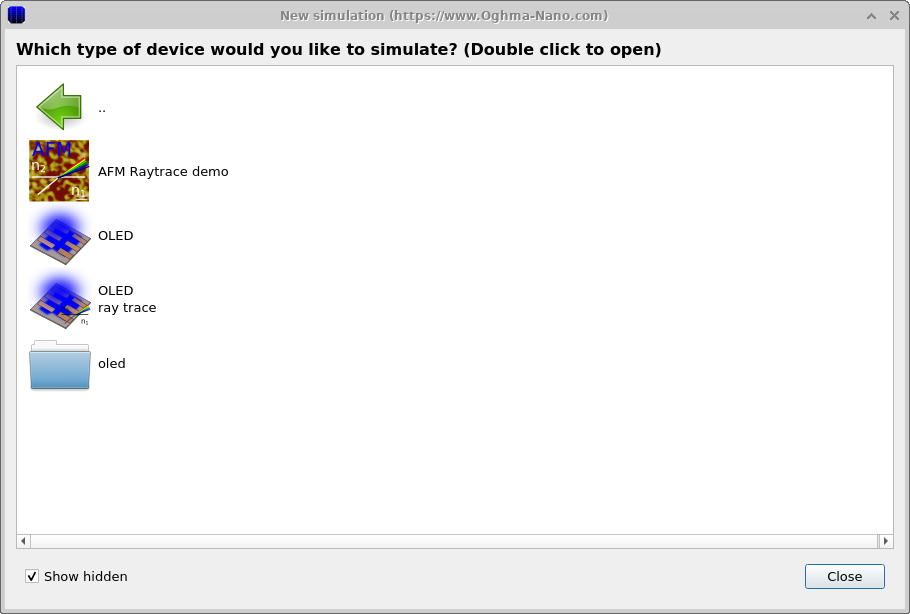
\includegraphics[width=0.5\textwidth,height=0.4\textwidth]{./images/oled/oled_new_sim.png}

&
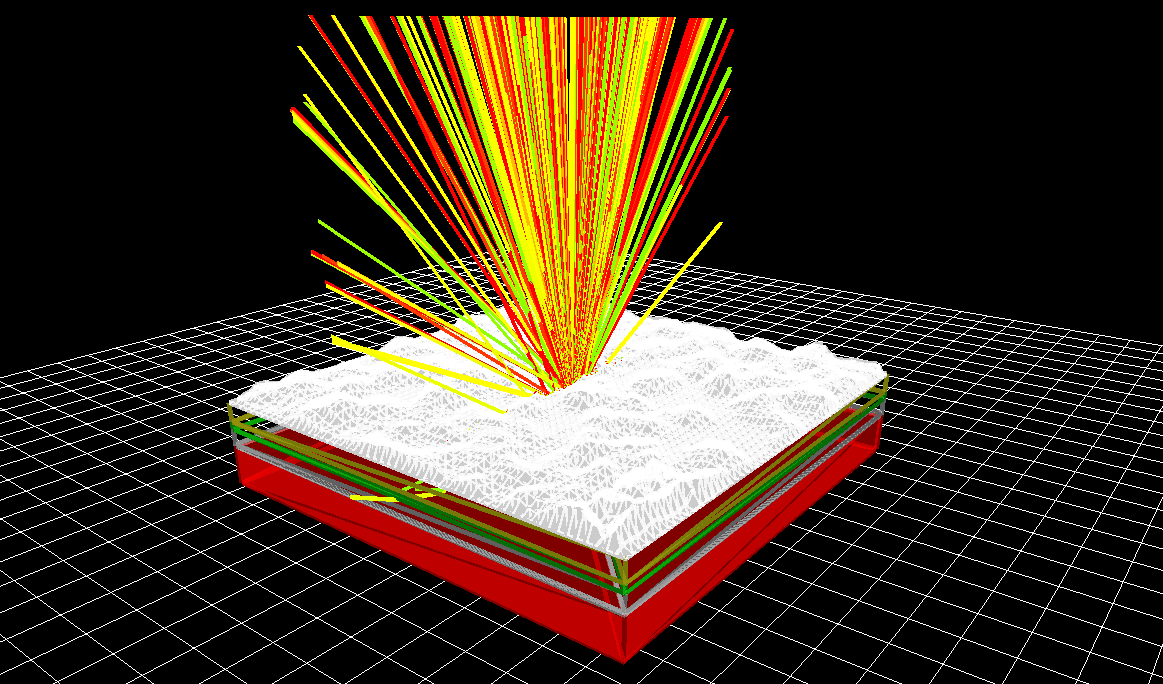
\includegraphics[width=0.5\textwidth,height=0.4\textwidth]{./images/oled/complex.png}

\\
\end{tabular}
\caption{a) The new simulation window; b) An example of an OLED ray trace simulation though a rough surface.}
\label{fig:oled5}
\end{figure}


\section{The spectrum of the emitted light}
Just as the electrical parameters can be set for each layer in the device so can the emission spectra. This is done in the \emph{emission parameters window} (see Figure \ref{fig:oled6}), which can be opened using the \emph{Emission parameters} button in the Device structure tab of the main window (see Figure \ref{ref:oled1}).  The emitted light spectrum can come from one of two sources. The first source is an experimental emission spectra which can be selected by changing the value of \emph{Experimental emission spectra} in \ref{fig:oled6}.  There are many spectra available in the materials data base but you can also add your own (see the section on databases).  By turning the option \emph{Use experimental emission spectra} to \emph{off}, one can use a numerically calculate emission spectra rather than an experimental one. The calculated emission spectra is calculated using Fermi's Golden rule from the carrier population and the DoS. This is only recommended for advanced users most users who are interested in OLED design should use .

If you have selected ray tracing in as the method to be used for outcoupling then for each layer one can select in what direction the rays are emitted. This is under the ray tracing heading visible in Figure \ref{fig:oled6}. The values define emission in terms of spherical coordinates theta and phi.  One can define the start and stop angles as well as the number of points use for both theta and phi. This enables one to study light escape as a function of angle. It is also worth noting for devices with flat surfaces one only needs to vary phi or theta but not both due to symmetry considerations.

The option \emph{emit from} will tell the ray tracer how to choose the position of the sources for each ray. The option visible in the window is \emph{At the Center of each emission layer}. If this option is selected the model will pick an emission point in the middle of each layer to start the ray tracing from, this is a good option if fast computational times are desired. Another option is \emph{At each electrical mesh point}, this will run the ray tracer at each electrical mesh point to accurately calculate emission probabilities, this can be slower although the decrease in speed can be mitigated against by increasing the number of threads the ray tracer runs on.

\begin{figure}[H]
\centering
\begin{tabular}{ c c }

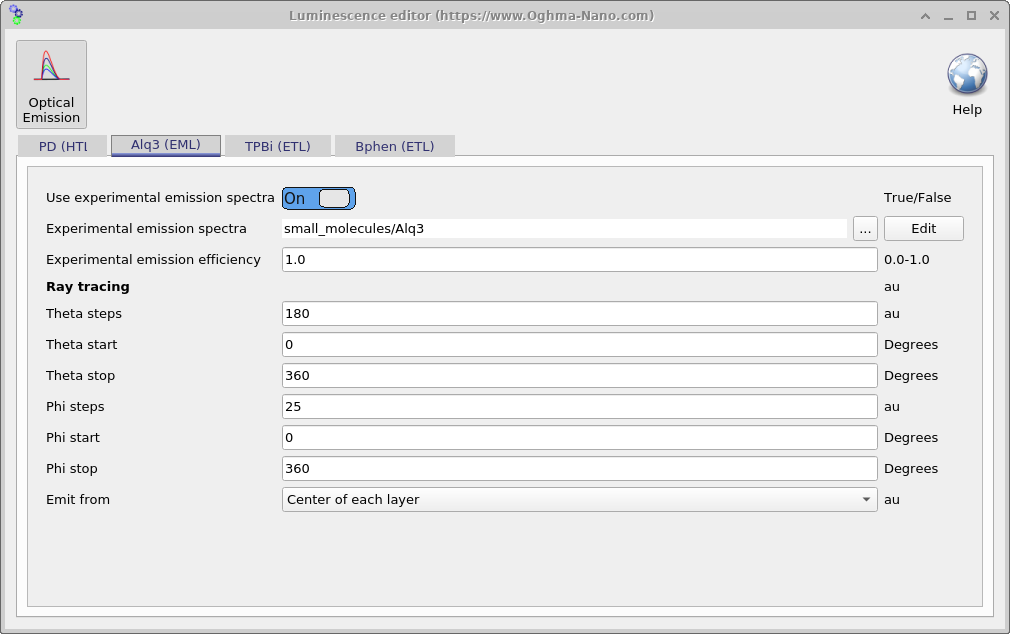
\includegraphics[width=0.5\textwidth,height=0.4\textwidth]{./images/oled/experimental_emission.png}

&
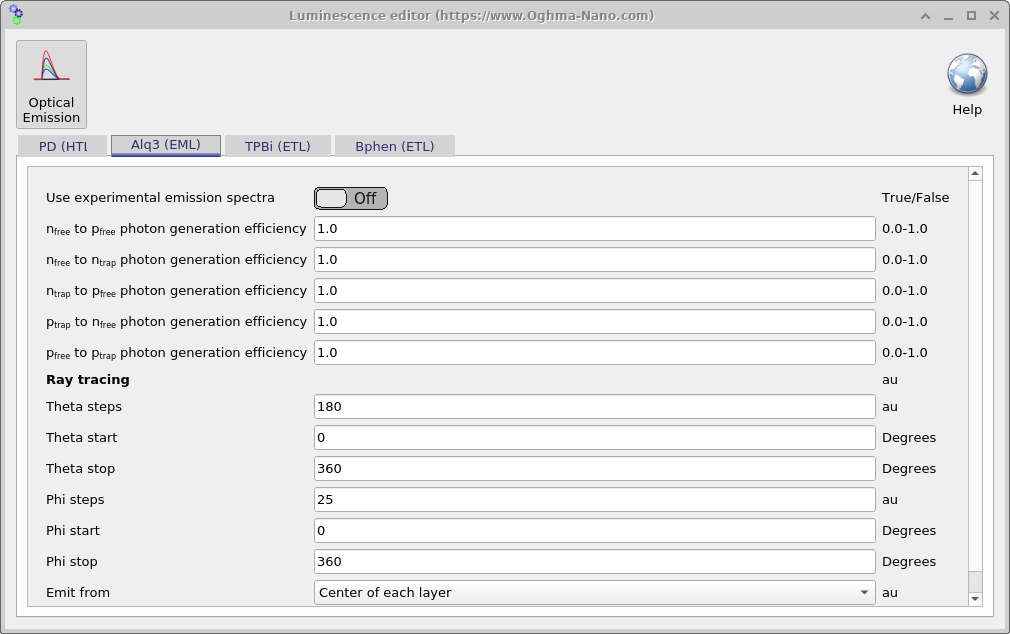
\includegraphics[width=0.5\textwidth,height=0.4\textwidth]{./images/oled/optical_emisson_dos.png}

\\
\end{tabular}
\caption{a) Using an experimental emission spectra; b) Calculating an emission spectra from the electrical density of states.}
\label{fig:oled6}
\end{figure}

\section{RGB, XYZ, CIE 1931 xyz colour spaces}
When designing OLED structures it is often important to understand how color of the emitted light changes as a function of viewing angle. When OghmaNano runs a ray tracing simulation it emits the files in table \ref{tab:oled_output1} which describe how the color of light changes as a function of viewing angle. These files are also visible in \ref{fig:oled7} as the colored colorspace icons.

\begin{table}[H]
\begin{center}
\begin{tabular}{ |c|l|c| } 
 \hline
	File name 			& 	Description  \\ 
 \hline
	$theta\_RGB.csv$			&	RGB values v.s. viewing angle \\ 
	$theta\_x.csv$			&	CIE 1931 x v.s. viewing angle \\ 
	$theta\_y.csv$			&	CIE 1931 y v.s. viewing angle \\ 
	$theta\_z.csv$			&	CIE 1931 z v.s. viewing angle \\
	$theta\_X.csv$			&	CIE 1931 X v.s. viewing angle \\ 
	$theta\_Y.csv$			&	CIE 1931 Y v.s. viewing angle \\ 
	$theta\_Z.csv$			&	CIE 1931 Z v.s. viewing angle \\ 
 \hline
\end{tabular}
\caption{Files describing the change of color with viewing angle.}
\label{tab:oled_output1}
\end{center}
\end{table}

\begin{figure}[H]
\centering
\begin{tabular}{ c c }

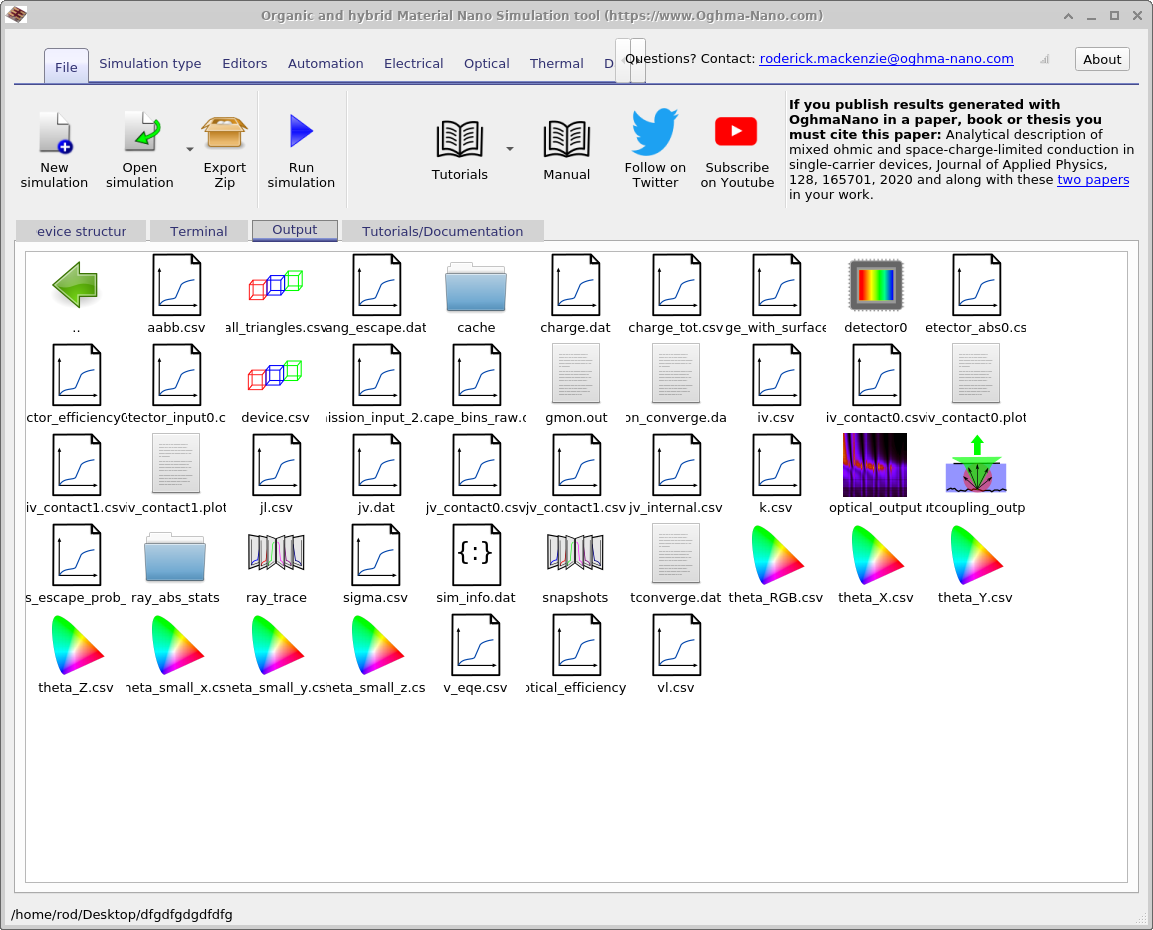
\includegraphics[width=0.7\textwidth,height=0.6\textwidth]{./images/oled/colors.png}

\\
\end{tabular}
\caption{The output of a simulation showing the files described in table \ref{tab:oled_output1}. These files are represented by the color space icons.}
\label{fig:oled7}
\end{figure}

\begin{figure}[H]
\centering
\begin{tabular}{ c }

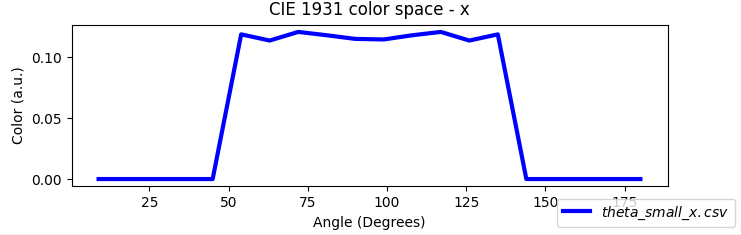
\includegraphics[width=0.9\textwidth,height=0.25\textwidth]{./images/oled/cie_x.png}

\\
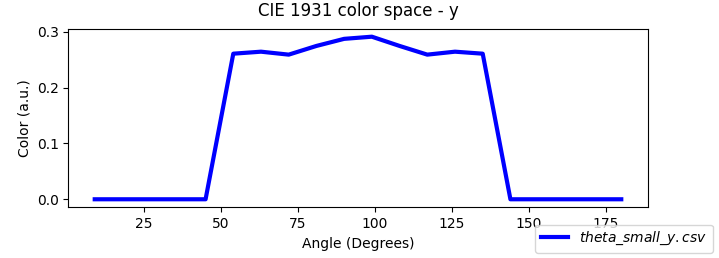
\includegraphics[width=0.9\textwidth,height=0.25\textwidth]{./images/oled/cie_y.png}

\\

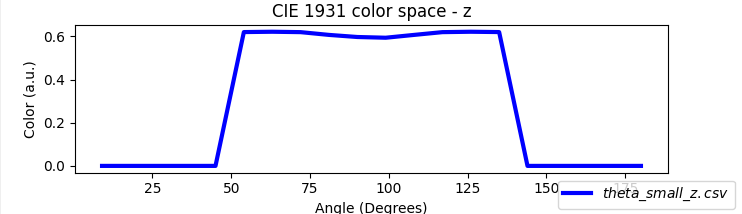
\includegraphics[width=0.9\textwidth,height=0.25\textwidth]{./images/oled/cie_z.png}
\\

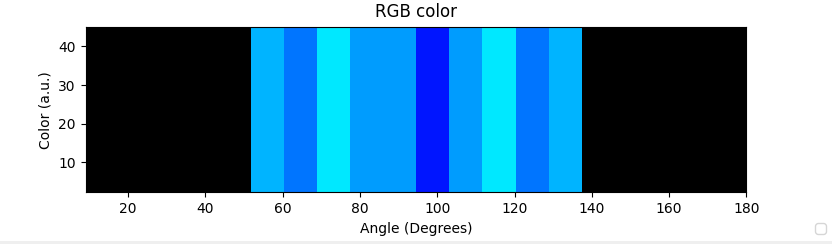
\includegraphics[width=0.9\textwidth,height=0.25\textwidth]{./images/oled/angle_vs_colors.png}
\\

\end{tabular}
\caption{Examples of color space output from OghamNano as a function of viewing angle; a) $theta\_x.csv$; b) $theta\_y.csv$; c) $theta\_z.csv$; and $theta_rgb.csv$}
\label{fig:oled8}
\end{figure}


